%% source: 2021-fa-midterm_01
%% tags: [binary search trees]
\begin{prob}
    Suppose the numbers
        \mintinline{python}{41},
        \mintinline{python}{32},
        and
        \mintinline{python}{40}
    are inserted (in that order) into the below binary search tree. Draw where
    the new nodes will appear.

    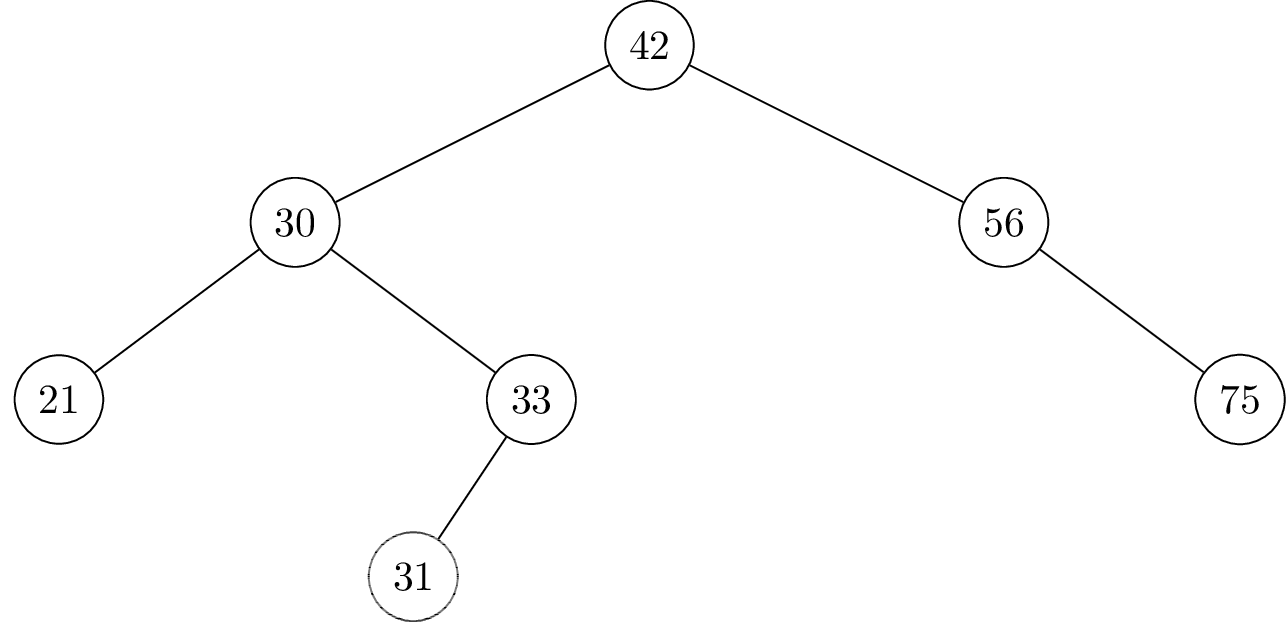
\includegraphics{./bst.png}

    \begin{soln}
        41 will be the right child of 33.

        32 will be the right child of 31.

        40 will be the left child of 41.


    \end{soln}

\end{prob}
